\documentclass[14pt,a4paper,titlepage]{extarticle}
\usepackage[utf8]{inputenc}
\usepackage[english,ukrainian]{babel}
\linespread{1.5} %полуторный межстрочный интервал
\usepackage[pdftex,left=2cm,right=1cm,top=2cm,bottom=2cm]{geometry} %поля
\pagestyle{myheadings} %номер страниц
\usepackage{indentfirst} %чтобы абзац после названия раздела был с красной строки
\parindent=1.25cm %красная строка 1,25см
\righthyphenmin=2 %чтобы 2 последние буквы слова переносились тоже
\sloppy %выривнивание по ширине
\usepackage{amssymb}
\usepackage{amsmath}
\usepackage{graphicx}
\graphicspath{{pictures/}}
\DeclareGraphicsExtensions{.png,.jpg}

\newcommand{\RomanNumeralCaps}[1]
    {\MakeUppercase{\romannumeral #1}}

\begin{document}
      \begin{titlepage}
      %\thispagestyle{empty}
         \begin{center}
ДНІПРОВСЬКИЙ НАЦІОНАЛЬНИЙ УНІВЕРСИТЕТ ІМ. О. ГОНЧАРА\\
ФАКУЛЬТЕТ ПРИКЛАДНОЇ МАТЕМАТИКИ\\
КАФЕДРА КОМП'ЮТЕРНИХ ТЕХНОЛОГІЙ\\
            \vspace{6cm}
            \bf Теоретична частина\\
            \bf до лабораторної роботи №2\\
            \bf <<ЧИСЕЛЬНЕ ІНТЕГРУВАННЯ>>\\
            \bf з курсу <<Методи обчислень>>\\
            \bf Варіант №2
        \end{center}
        \vspace{3cm}
        \begin{flushright}
Виконав:\\
студент групи ПА-18-1(2)\\
Лєшанов Андрій
        \end{flushright}
        \begin{center}
        \vspace{4.5cm}
        Дніпро\\
         2020
        \end{center}
   \end{titlepage}
\setcounter{page}{2}
\newpage
{\centering\bf\large Теория\par}

{\bf 1. Постановка задачи численного интегрирования.}

Будем рассматривать задачу вычисления опрегделенного интеграла $ \ int \ limits_a ^ b F (x) \, dx, $ где $ [a, \, b] $ - задач конечной промежуток числовои оси, $ F (x) $ - заданная функция на $ [a, \, b]. $ Геометрическое согдержание такого интеграла заключается в том, что его значение равно площади криволинейной трапеции, ограниченной графиком функции
$ Y = F (x) $ и прямыми $ y = 0, \ x = a, \ x = b. $

Под численным интегрированием понимают приближенное вычисление интеграла. Если подынтегральная функция $ F (x) $ имеет сложное аналитическое выражение или задана таблично на $ [a, \, b], $ то точные методы интегрирования, которые изучаются в математических анализе, становятся неиспользуемыми. Для таких интегралов разрабатывают приближенные способы вычисления.

Квадратурные формулы - формула приближения вычисления интеграла.

Основная игдея построения квадратурных формул основана на приближенной замене подынтегральной функции некоторой другой функцией, интеграл от которой легко вычислить.

Простейшие квадратурные формулы могут быть получены из геометрических соображений.

{\ Centering \ includegraphics {2} \ par}
Если заменить участок кривой $ y = F (x) $ в $ [a, \, b] $ прямой $ AB, $ где $ A (a, \, F (a) $ и $ B (b, \, F ( b), $ то получем квадратурные формулы трапеции:
$$ \ int \ limits_a ^ b F (x) \, dx \ approx (b-a) \ cdot \ frac {F (a) + F (b)} {2}. $$
При этом площади заштрихованих на рисунке фигур, взяты с соответствующим знаком, в сумме образуют погрешность этой приблеженной формулы.

Любую квадратурнуюю формулу можно записать в следующем наиболее общем оте:
\begin{equation}
\int\limits_a^b p(x)\cdot f(x)\, dx = \sum_{i=0}^n A_i\cdot f(x_i)+R_n(f),
\end{equation}
где $n\in \mathbb{Z}_0$ выбирается из соображений точности ($\mathbb{Z}_0$ - множество этолых неотрицательных чисел); $A_i,\ i=\overline{0,\, n}$ - квадратурные коэффициенти;  $x_i,\ i=\overline{0,\, n}$ - квадратурные узлы; $R_n(f)$ - остаточный член (погрешность) квадратурной формулы; $p(x)$ - известная (так называемая "весовая") функция, которая согдержит в себе "особенности"
\\подынтегральной функции; $f(x)$ - известная гладкая функция на $[a,\, b].$

Разные квадратурные формулы отличаются способом выбора квадратурных узлов $x _ i, i=\overline{0, n}$ и коэффициентов $A _ i, i=\overline{0,n}$ при заданном $n\in \mathbb{Z} 0.$ Узлы и коэффициенты квадратурной формулы избирают или при условии кстижения повышенной точности результата, или по соображениям простоты и укбства вычислений.

Квадратурную формулу (1) называют точной, если $R_n(f)\equiv 0.$


Большинство квадратурных формул основано на приближенной замене подынтегральной функции алгебраическим многочленом. В свясо с этем возникло понятие алгебраической степени точности квадратурной формулы.

Квадратурнаяя формула (1) имеет алгебраческую степень точности $m$, если она точна ($R_n(f)=0$) для всех алгебраических многочленов степени $\leqslant m$ и не является точной хотя бы для одного алгебраического многочлена степени $m+1.$\\
Следует ожидать, что чем выше алгебраическая степень квадратурной формулы, тем
более точный результат она будет давать на классе непрерывных функций. Если квадратурная формула точна для всех алгебраических многочленов степени $m$, то она будет точна и для всех алгебраических многочленов степени $<m.$

{\bf 2. Интерполяционные квадратурные формулы.}

Построение интерполяционных квадратурных формул основана на замене подынтегральнйї функэти ее интерполяционным многочленом.

Выберем на отрезке интегрированния $[a,\, b]$ совокупность попарно различных точек $a\leqslant x_0<x_1\ldots <x_n\leqslant b$ (узлов интерполяции) и представим подынтегральную функцию $f(x)$ в виде суми ее интерполяционного многочлена и остаточного члена:
$$f(x)=L_n(x)+R_n(x),\ \forall x\in [a,\, b].$$

В качестве интерполяционного многочлена будетм рассматривать многочлен Лагранжа:
$$L_n(x)=\sum_{i=0}^n f(x_i)\cdot\prod_{\genfrac{}{}{0pt}{}{j=0}{j\neq i}}^n\frac{x-x_j}{x_i-x_j};\ R_n(x)=\frac{1}{(n+1)!}\cdot f^{(n+1)}(\xi)\cdot \omega _{n+1}(x),$$
$$\xi=\xi (x)\in [a,\, b],$$
где $\omega _{n+1}(x) =(x-x_0)\cdot (x-x_1)\cdot\ldots\cdot (x-x_n),\ \forall x\in [a,\, b].$

Тогда: 
$$\int\limits_a^b p(x)\cdot f(x)\, dx=\int\limits_a^b p(x)\cdot (L_n(x)+R_n(x))\, dx=$$
$$=\int\limits_a^b p(x)\cdot L_n(x)\, dx+\int\limits_a^b p(x)\cdot R_n(x)\, dx=$$
$$=\int\limits_a^b p(x)\cdot\sum_{i=0}^n f(x_i)\cdot\prod_{\genfrac{}{}{0pt}{}{j=0}{j\neq i}}^n\frac{x-x_j}{x_i-x_j}\, dx+\int\limits_a^b p(x)\cdot\frac{1}{(n+1)!}\cdot f^{(n+1)}(\xi)\cdot \omega _{n+1}(x)\, dx=$$
$$
=\sum_{i=0}^n f(x_i)\cdot\int\limits_a^b p(x)\cdot\prod_{\genfrac{}{}{0pt}{}{j=0}{j\neq i}}^n\frac{x-x_j}{x_i-x_j}\, dx+\frac{1}{(n+1)!}\cdot\int\limits_a^b p(x)\cdot f^{(n+1)}(\xi)\cdot \omega _{n+1}(x)\, dx.
$$

Квадратурная формула (1), в которой квадратурные узлы $x_0, x_1,\ldots, x_n$ совпадают с узлами интерполяции, а коэффициенты вычисляются по формуле:
\begin{equation}
A_i=\int\limits_a^b p(x)\cdot\prod_{\genfrac{}{}{0pt}{}{j=0}{j\neq i}}^n\frac{x-x_j}{x_i-x_j}\, dx,\ i=\overline{0,\, n},
\end{equation}
называется интерполяционной.\\
{\bf Теорема.} Для того, чтобы квадратурная формула (1) была точна для любого многочлена степени $n$, необходимо и кстаточно, чтобы она была интерполяционной. А это значит, что алгебраическая степень точности интерполяционной квадратурной формулы равен, как минимум, $n$.

Пусть подынтегральная функция $f(x)$ непрерывна на $[a,\, b]$ вместе со своими производными к $(n+1)$-го порядка включительно, причём существует константа $M$:\\$M=\underset{a\leqslant x\leqslant b}{max}\left| f^{(n+1)}(x)\right|.$ Тогда получем оценку:
$$\left| R_n(f)\right|\leqslant\frac{1}{(n+1)!}\int\limits_a^b\left| p(x)\cdot f^{(n+1)}(\xi)\cdot\omega _{n+1}(x)\right| dx\leqslant\frac{M}{(n+1)!}\int\limits_a^b\left| p(x)\cdot\omega _{n+1}(x)\right| dx.$$

Оценка погрешности может быть существенно завышена, потому что, если функция\\ $p(x)\cdot\omega _{n+1}(x)$ меняет знак на $[a,\, b]$, то истинная величина погрешности может быть намного меньше, чем правая часть неравенства.

{\bf 3. Квадратурная формула Ньютона-Котеса.}

Квадратурная формула Ньютона-Котеса является особым случаем интерполяционной квадратурной формулы (1). Пусть:

1) $p(x)\equiv 1$ на $[a,\, b]$; 

2) квадратурные узлы $x_0, x_1,\ldots, x_n$ равноудалены с шагом $h$:
\begin{equation}
x_i=a+i\cdot h,\ i=\overline{0,\, n};\ h=\frac{b-a}{n},
\end{equation}
при этом $x_0=a,\ x_n=b;$

3) промежуток $[a,\, b]$ конечный.

Выполним у формулы (2) замену переменной интегрирования: 
\begin{equation}
x=x_0+t\cdot h
\end{equation}
и перейгдем от $x\in [a,\, b]$ к новой переменной $t\in [0,\, n].$ Получем: $dx=h\cdot dt;$
$$
\prod_{\genfrac{}{}{0pt}{}{j=0}{j\neq i}}^n (x-x_j)=(x-x_0)(x-x_1)\ldots (x-x_{i-1})(x-x_{i+1})\ldots (x-x_n)=\{\text{врах. (3), (4)}\}=
$$
$$
=(x_0+th-x_0)(x_0+th-(x_0+h))\ldots (x_0+th-(x_0+(i-1)h))(x_0+th-(x_0+(i+1)h))\ldots
$$
$$
\ldots (x_0+th-(x_0+nh))=h^n\cdot t(t-1)\ldots (t-i+1)(t-i-1)\ldots (t-n);
$$
$$
\prod_{\genfrac{}{}{0pt}{}{j=0}{j\neq i}}^n (x_i-x_j)=(x_i-x_0)(x_i-x_1)\ldots (x_i-x_{i-2})(x_i-x_{i-1})(x_i-x_{i+1})(x_i-x_{i+2})\ldots (x_i-x_n)=
$$
$$
=\{\text{врах. (3)}\}=(x_0+ih-x_0)(x_0+ih-(x_0+h))\ldots (x_0+ih-(x_0+(i-2)h))\cdot
$$
$$
\cdot (x_0+ih-(x_0+(i-1)h))(x_0+ih-(x_0+(i+1)h))(x_0+ih-(x_0+(i+2)h))\ldots 
$$
$$
\ldots (x_0+ih-(x_0+nh))=h^n\cdot i(i-1)\ldots 2\cdot 1\cdot (-1)\cdot (-2)\ldots (-(n-i))=
$$
$$
=h^n\cdot i!(-1)^{n-i}\cdot (n-i)!.
$$

Подставив в формулу для $A_i,\ i=\overline{0,\, n},$ получаем:
$$
A_i=\int\limits_0^n\frac{h^n\cdot t(t-1)\ldots (t-i+1)(t-i-1)\ldots (t-n)}{h^n\cdot i!(-1)^{n-i}\cdot (n-i)!}\cdot h\, dt=
$$
$$
=\frac{b-a}{n}\cdot\frac{(-1)^{n-i}}{i!\cdot (n-i)!}\int\limits_0^n t(t-1)\ldots (t-i+1)(t-i-1)\ldots (t-n)\, dt=
$$
\begin{equation}
=(b-a)\cdot B_i,\ i=\overline{0,\, n},
\end{equation}
где
\begin{equation}
B_i=\frac{(-1)^{n-i}}{n\cdot i!\cdot (n-i)!}\int\limits_0^n t(t-1)\ldots (t-i+1)(t-i-1)\ldots (t-n)\, dt,\ i=\overline{0,\, n}.
\end{equation}

Квадратурные коэффициенты $B_i,\ i=\overline{0,\, n}$, которые определяются по формулам (6), называют коэффициентами Котеса.

подставляя в квадратурную формулу (1) вместо узлов и коэффициентов их выражения по формулам (3) и (5) соответственно, получаем:
\begin{equation}
\int\limits_a^b f(x)\, dx=(b-a)\cdot \sum_{i=0}^n B_i\cdot f(a+ih)+R_n(f).
\end{equation}

Интерполяционная квадратурная формула (7) с равноудалеными узлами называется квадратурной формулой Ньютона-Котеса. 


Иногда для укбства рассмотрения формулу Ньютона-Котеса записівают в виде
$$
\int\limits_a^b f(x)\, dx\approx (b-a)\cdot \sum_{i=0}^n B_i\cdot f(a+ih).
$$

Коэффициенты Котеса имеют следующие важные свойства:

1) коэффициенты Котеса не зависят от промежутка интегрирования и величины шага;

2) коэффициенты Котеса, симетричны видносительно середины промежутка, равны между собой;

3) сума коэффициентов Котеса при любом $n\in \mathbb{Z}_0$ равняется  еденице.

{\bf 4. Квадратурные формулы прямоугольников.}

Запишем квадратурную формулу Ньютона-Котеса в виде
$$
\int\limits_a^b f(x)\, dx\approx (b-a)\cdot \sum_{i=0}^n B_i\cdot f(a+ih),\eqno(1)
$$
$$
B_i=\frac{(-1)^{n-i}}{n\cdot i!\cdot (n-i)!}\int\limits_0^n t(t-1)\ldots (t-i+1)(t-i-1)\ldots (t-n)\, dt,\ i=\overline{0,\, n}.\eqno(2)
$$

Остаточный член этой квадратурной формулы имеет вид
$$
R_n(f)=\frac{1}{(n+1)!}\cdot\int\limits_a^b f^{(n+1)}(\xi)\cdot \omega _{n+1}(x)\, dx,\ \xi=\xi (x)\in [a,\, b],\eqno(3)
$$

При $n=0$ имеем у квадратурной формулы (1) только один узел $x_0\in [a,\, b]$ и один коэффициент $B_0.$ При этом формулой (2) для вычисления коэффициентов Котеса пользоваться нельзя, так как она содержит неопределенность (деление на нуль). Потому, исходя из общей идеи построения интерполяционной квадратурной формулы, заменим
подынтегральную функцию $f(x)$ ее интерполяционным многочленом, построенным по
одному узлу $x_0\in [a,\, b].$ Такой многочлен имеет  нулевую степень и,
согласно с условием интерполяции, равняется  $L_0(x)\equiv f(x_0),\ \forall x\in [a,\, b].$ Положим
$$
f(x)\approx L_0(x)\Longleftrightarrow f(x)\approx f(x_0),\ \forall x\in [a,\, b].
$$

Тогда $\int\limits_a^b f(x)\, dx\approx\int\limits_a^b f(x_0)\, dx=f(x_0)\int\limits_a^b dx=f(x_0)\cdot (b-a).$

Квадратурная формула 
$$
\int\limits_a^b f(x)\, dx\approx f(x_0)\cdot (b-a)\eqno(4)
$$
называется элементарной квадратурной формулой прямоугольников.

Если $x_0=a,$ то формула (4) называется элементарной формулой левых прямоугольников, при $x_0=b$ - элементарной формулой правых прямоугольников, при $x_0=\dfrac{a+b}{2}$ - элементарной формулой средних прямоугольников.

Рассмотрим погрешность элементарной формулы левых прямоугольников. По определению, $R_0(x)=\int\limits_a^b f(x)\, dx -(b-a)\cdot f(a).$ С другой стороны, из общей формулы (3) при $n=0,\ x_0=a$ имеем $R_0(f)=\int\limits_a^b f'(\xi)\cdot (x-a)\, dx.$ Так как, по предположению, $f'(\xi)$ непрерывна на $[a,\, b],$ а функция $(x-a)$ 
сохраняет  знак на $[a,\, b],$ то, на основании теоремы про среднее  значение, найдется точка $\eta\in [a,\, b]$ такая, что
$$
R_0(f)=f'(\eta)\cdot\int\limits_a^b (x-a)\, dx=\left. f'(\eta)\cdot\frac{(x-a)^2}{2}\right| _a^b=\frac{(b-a)^2}{2}\cdot f'(\eta),\ \eta\in [a,\, b].\eqno(5)
$$

Формула (5) дает  выражение для остаточного члена элементарной квадратурной формулы левых прямоугольников. Формула остаточного члена элементарной формулы правых
прямоугольников сходится с формулой (5) с точностью к знака:
$$
R_0(f)=-\frac{(b-a)^2}{2}\cdot f'(\eta),\ \eta\in [a,\, b].\eqno(6)
$$

Рассмотрим остаточный член элементарной формулы средних прямоугольников.

{\centering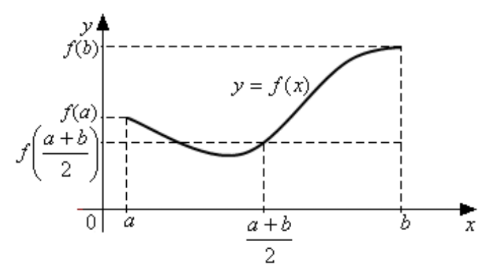
\includegraphics{3}\par}

По определению, в этом случае $R_0(f)=\int\limits_a^b f(x)\, dx -(b-a)\cdot f\left( \dfrac{a+b}{2}\right).$ С другой стороны, с общей формулы (3) при $n=0,\ x_0=\dfrac{a+b}{2}$ имеем\\
$R_0(f)=\int\limits_a^b f'(\xi)\cdot \left( x-\dfrac{a+b}{2}\right)\, dx.$ К последнему интегралу уже нельзя использовать теорему про среднее  значение, так как функция $x_0=\dfrac{a+b}{2}$ меняет знак на $[a,\, b].$

Разложим функцию $f(x)$ в ряд Тейлора в окресности точки $x_0=\dfrac{a+b}{2}:$
$$
f(x)=f\left(\frac{a+b}{2}\right) +f'\left(\frac{a+b}{2}\right)\left( x-\frac{a+b}{2}\right)+\frac{f''(\overset{\sim}{x})}{2!}\left( x-\frac{a+b}{2}\right) ^2,
$$
$$
\overset{\sim}{x}=x_0+\Theta (x-x_0),\ 0<\Theta <1.
$$

Перенесем в левую часть $f\left(\dfrac{a+b}{2}\right)$ и проинтегрируем на промежутке $[a,\, b]$:
$$
\int\limits_a^b f(x)\, dx-\int\limits_a^b f\left(\frac{a+b}{2}\right)\, dx=
$$
$$
=\int\limits_a^b f'\left(\frac{a+b}{2}\right)\left( x-\frac{a+b}{2}\right)\, dx+\int\limits_a^b \frac{f''(\overset{\sim}{x})}{2!}\left( x-\frac{a+b}{2}\right) ^2 dx;
$$
$$
\int\limits_a^b f(x)\, dx-f\left(\frac{a+b}{2}\right) (b-a)=f'\left(\frac{a+b}{2}\right)\cdot\frac{1}{2}\left. \left( x-\frac{a+b}{2}\right) ^2\right| _a^b+
$$
$$
+\frac{1}{2}\int\limits_a^b f''(\overset{\sim}{x})\left( x-\frac{a+b}{2}\right) ^2dx.
$$

Левая часть, по определению, является  $R_0(f)$; в правой же части первое слагаемое равняется  нулю, а к второму слагаемому можно использовать теорему про среднее  значение. Тогда
$$
R_0(f)=\frac12\, f''(\eta)\cdot\int\limits_a^b \left( x-\frac{a+b}{2}\right) ^2 dx=\frac16\, f''(\eta)\cdot\left.\left( x-\frac{a+b}{2}\right) ^3\right|_a^b=
$$
$$ 
=\frac{1}{24} (b-a)^3 f''(\eta),\ \eta\in [a,\, b].\eqno(7)
$$

Формула (7) дает  выражение для остаточного члена элементарной квадратурной формулы средних прямоугольников.

Если длина отрезка $[a,\, b]$ велика, то рассматреваемые элементарные квадратурные
формулы имеют невысокую точность. В этом случае используют так называемые обобщенные квадратурные формулы. Отрезок интегрирования $[a,\, b]$ делят на достаточно большое число $N>0$ равных частей с шагом $h=\dfrac{b-a}{N}$ точками $x_k=a+kh,\ k=\overline{0,\, N}$, и на каждом частичном промежутке $[x_k,\ x_{k+1}],\ k=\overline{0,\, N-1}$ используют ту или иную элементарную квадратурную формулу, а потом результаты суммируют по всем значениям $k=\overline{0,\, N-1}$.

Например, Использование элементарной формулы левых прямоугольников дает :
$$
\int\limits_{x_k}^{x_{k+1}} f(x)\, dx\approx h\cdot f(x_k),\ k=\overline{0,\, N-1}.
$$

Суммирование таких приближенных равенств по всем $k=\overline{0,\, N-1}$ приводит к обобщенной квадратурной формуле левых прямоугольников
$$
\int\limits_a^b f(x)\, dx\approx h\cdot\sum_{k=0}^{N-1} f(x_k).\eqno(8)
$$

Аналогично можно построить другие обобщенные квадратурные формулы:
\begin{itemize}
\item правых прямоугольников
$$
\int\limits_a^b f(x)\, dx\approx h\cdot\sum_{k=1}^N f(x_k);\eqno(9)
$$
\item средних прямоугольников
$$
\int\limits_a^b f(x)\, dx\approx h\cdot\sum_{k=0}^{N-1} f\left(\frac{x_k+x_{k+1}}{2}\right).\eqno(10)
$$
\end{itemize}

Остаточные члены обобщенных квадратурных формул прямоугольников (8) - (10)
получают в результате суммирования остатков для каждого из частичных промежутков $[x_k,\ x_{k+1}],\ k=\overline{0,\, N-1}$. Формули остаточных членов имеют вид:
\begin{itemize}
\item для обобщенной формулы левых прямоугольников (8)
$$
R_0^{(N)} (f)=\frac12\frac{(b-a)^2}{N} f'(\xi)=O(h),\ \xi\in [a,\, b];\eqno(11)
$$
\item для обобщенной формулы правых прямоугольников (9)
$$
R_0^{(N)} (f)=-\frac12\frac{(b-a)^2}{N} f'(\xi)=O(h),\ \xi\in [a,\, b];\eqno(12)
$$
\item для обобщенной формулы средних прямоугольников (10)
$$
R_0^{(N)} (f)=\frac{1}{24}\frac{(b-a)^3}{N} f''(\xi)=O(h^2),\ \xi\in [a,\, b].\eqno(13)
$$
\end{itemize}

Из формул (11) - (13) для остаточных членов обобщенныех квадратурных формул видно, что чем меньше величина шага $h$, тем меньше погрешность численного интегрирования. При этом, сравнивая остаточные члены по формулам (11) - (13), можно заметить, что порядок их точности одинаковый для формул левых и правых прямоугольников (первый порядок точности по $h$), а формула средних прямоугольников имеет  более високую точность (второй порядок точности по $h$), т. е. при одинаково маленьком $h$ формула средних прямоугольников даст более точный результат.

Кроме того, формулы левых и правых прямоугольников будуть точными только для $f(x)=const$, в то же время как формула средних прямоугольников будет точной для любой линейной функции (многочлена первой степени). Остюда выплывает , что алгебраическая степень точности квадратурных формул левых и правых прямоугольников равняется  0, а алгебраическая степень точности формулы средних прямоугольников равняется  1.

{\bf 5. Квадратурные формулы трапеций.}

При $n=1$ имеем у квадратурной формулы Ньютона-Котеса (1) два узла на $[a,\, b]:\ x_0=a,\ x_1=b$ и два коэффициента $B_0=B_1=\dfrac12$, так что из (1) сразу получаем
$$
\int\limits_a^b f(x)\, dx\approx\frac{b-a}{2}\cdot (f(a)+f(b)).\eqno(14)
$$

Квадратурная формула (14) называется элементарной квадратурной формулой трапеции.


Ее остаточный член выводится из общей формулы (3) с использованием теоремы
про среднее  значение:
$$
R_1(f)=\frac{1}{2!}\int\limits_a^b f''(\xi)(x-a)(x-b)dx=\frac12 f''(\eta)\int\limits_a^b (x-a)(x-b)dx=
$$
$$
=-\frac{1}{12} (b-a)^3 f''(\eta),\ \eta\in [a,\, b].\eqno(15)
$$

Разобьем отрезок $[a,\, b]$ на $N>0$ равных частей с шагом $h=\dfrac{b-a}{N}$ точками $x_k=a+kh,\ k=\overline{0,\, N}$. На каждом частичном промежутке $[x_k,\ x_{k+1}],\ k=\overline{0,\, N-1}$ используем элементарную формулу трапеции (14):
$$
\int\limits_{x_k}^{x_{k+1}} f(x)\, dx\approx\frac{h}{2}(f(x_k)+f(x_{k+1})),\ k=\overline{0,\, N-1}.
$$

Просуммируем эти приближенные равенства по всем значениям $k=\overline{0,\, N-1}$:
$$
\int\limits_a^b f(x)\, dx\approx\frac{h}{2}\left[ f(x_0)+f(x_1)+f(x_1)+f(x_2)+\ldots +f(x_{N-2})+f(x_{N-1})+f(x_{N-1})+\right.$$
$$
+\left. (x_N)\right],
$$
или
$$
\int\limits_a^b f(x)\, dx\approx\frac{h}{2}(f(x_0)+f(x_N))+h\sum_{k=1}^{N-1} f(x_k).\eqno(16)
$$

Это так называемая обобщенная квадратурная формула трапеций. Ее остаточный член получают в результатк суммирования остатков по частичным промежуткам $[x_k,\ x_{k+1}],\ k=\overline{0,\, N-1}$:
$$
R_1^{(N)}(f)=-\frac{1}{12}\cdot\frac{(b-a)^3}{N^2} f''(\xi)=O(h^2),\ \xi\in [a,\, b].
\eqno(17)
$$

Сравнивая формулы остаточных членов (17) и (13) видим, что квадратурные формулы трапеций и средних прямоугольников имеют одинаковый, второй порядок точности по $h$, а также одинаковую алгебраическую степень точности, равную 1.


\textbf{6. Квадратурные формулы наивысшей алгебраической степени точности}


При $n=2$ имеем в квадратурной формуле Ньютона Котеса (1) три узла на $[a,\, b]:\ x_0=a,\ x_1=\dfrac{a+b}{2},\ x_2=b$ а три коэффициента $B_0=B_2=\dfrac16,\ B_1=\dfrac46$, так что из (1) сразу получаем
$$
\int\limits_a^b f(x)\, dx\approx\frac{b-a}{6}\left( f(a)+4f\left(\frac{a+b}{2}\right)+f(b)\right).
\eqno(18)
$$

Квадратурная формула (18) називается элементарной квадратурной формулой Симпсона (парабол).

Геометрический смысл формулы Симпсона (18) состоит в том, что участок кривой $y=f(x)$ на $[a,\, b]$ заменяется параболой, которая проходит через три точки $A_0,\ A_1,\ A_2$: $A_i(x_i,\, f(x_i)),\ i=\overline{0,\, 2}.$

Остаточный член  элементарной квадратурной формулы Симпсона имеет вид
$$
R_2^{(N)}(f)=-\frac{1}{90}\frac{(b-a)^5}{2}f^{\text{(\RomanNumeralCaps{4})}}(\eta),\ \eta\in [a,\, b].
\eqno(19)
$$

Для построения обобщенной формулы Симпсона разобьем отрезок интегрирования $[a,\, b]$ на четное число $N>0$ равных частей с шагом $h=\dfrac{b-a}{N}$ точками $x_k=a+kh,\ k=\overline{0,\, N}$. На каждом частичном промежутке $[x_{k-1},\ x_{k+1}],\ k=1,\ 3,\ 5,\ldots ,\ N-1$, которые содержат три точки $x_{k-1},\ x_k,\ x_{k+1}$, используем элементарную формулу Симпсона (18):
$$
\int\limits_{x_{k-1}}^{x_{k+1}} f(x)\, dx\approx\frac{2h}{6}(f(x_{k-1})+4f(x_k)+f(x_{k+1})).
$$

Просуммировав эти приближенные равенства по нечетным $k=1,\ 3,\ 5,\ldots ,\ N-1$, получим:
$$
\int\limits_a^b f(x)\approx\frac{h}{3}\left[ f(x_0)+f(x_N)+4\left( f(x_1)+f(x_3)+\ldots+f(x_{N-1})\right)\right.+
$$
$$
\left. +2\left( f(x_2)+f(x_4)+\ldots +f(x_{N-2})\right)\right].\eqno(20)
$$

Это и есть обобщенная квадратурная формула Симпсона. Ее остаточный член получают в результате суммирования остатков по промежуткам $[x_{k-1},\ x_{k+1}],\ k=1,\ 3,\ 5,\ldots ,\ N-1$:
$$
R_2^{(N)}(f)=-\frac{1}{180}\frac{(b-a)^5}{N^4} f^{\text{(\RomanNumeralCaps{4})}} (\xi)=O(h^4),\ \xi\in [a,\, b].\eqno(21)
$$

Замечание 1. Из построения формулы Симпсона следует, что она (как частный случай интерполяционной квадратурной формулы при $ n = 2 $) точна для всех многочленов второй степени. Из формул остаточных членов (19) и (21) видно, что она будет точной и для многочленов третьей степени. Итак, алгебраический степень точности квадратурной формулы Симпсона равен 3.

Замечание 2. Из рассмотренных нами квадратурных формул наиболее точной является формула Симпсона. Однако отсюда не следует, что в конкретных случаях более грубая формула не может дать лучших результатов, чем более точна. Точность квадратурной формулы существенно зависит от расположения узлов. Если подынтегральная функция $ f (x) $ имеет значительное количество нулей или экстремумов, то в этом случае шаг интегрирования $ h $ следует выбирать так, чтобы он был намного меньше расстояний между соседними нулями и экстремумами функции.





\textbf{7. Квадратурные формулы наивысшей алгебраической степени точности}


Интерполяционные квадратурные формулы имеют степень по меньшей мере $n$. Отсюда возникает вопрос: существуют ли квадратурные формулы более высокой степени точности и какова наивысшая степень точности квадратурных формул. \\
Общая квадратурная формула
\begin{equation}
\int\limits_a^b p(x)\cdot f(x)dx = \sum_{k = 0}^n A_k \cdot f(x_k) + R_n(f)
\label{(1)}
\end{equation}
при фиксированном $n \in \mathbb{Z} $ имеет $(2n + 1)$ параметра: $(n+1)$ квадратурных узлов $x_k$, $k = \overline{0,n}$ и $(n+1)$ квадратурных коэффициентов $A_k$, $k = \overline{0,n}$. Поэтому пусть (1) будет точной для $( R_n ( f ) = 0 )$ для всех алгебраических многочленов до степени $(2n + 1)$ включительно, т. е.
\begin{equation}
\int\limits_a^b p(x)\cdot x^idx = \sum_{k = 0}^n A_k \cdot x_k^i,\quad i = 0, 1, \ldots, 2n+1
\label{(2)}
\end{equation}
На (2) можно смотреть как на систему $(2n+2)$ нелинейных алгебраических уравнений относительно $(2n+2)$ неизвестных $x_k$ и $A_k$, $k = \overline{0,n}$. Если решение такой системы существует, то квадратурная формула степени $(2n+1)$ может быть построена.
\\
\\
\textit{{\textbf{Теорема 1}}}
Квадратурнаяя формула (1) точная для всех многочленов степени не выше $(2n+1) \Leftrightarrow$ 
\begin{enumerate}
   \item чтобы она была интерполяционной
   \begin{equation}
		A_k = \int\limits_a^b p(x)\cdot \prod_{\genfrac{}{}{0pt}{}{j=0}{j\neq k}}^n \frac{x - x_j}{x_k - x_j} dx, \quad k = \overline{0,n}
		\label{(3)}
	\end{equation}
	где $x_i, \ i = \overline{0,n}$ являются узлами интерполяции;
	\item чтобы многочлен $\omega_n+1 (x) = (x-x_1)\ldots(x - x_n)$ был ортогонален с весом $p(x)$
	на отрезке $\left[  a, b\right] $ к любому алгебраическому многочлену $Q_n(x)$ степени не выше $n$, 
	\begin{equation}
		\int\limits_a^b p(x)\cdot \omega_n+1 (x) \cdot Q_n(x) dx = 0
		\label{(4)}
	\end{equation}
   \end{enumerate}
   Из теоремы 1 $\Rightarrow$ алгоритм	построения квадратурной формулы
алгебраической степени точности $(2n+1)$:
\begin{enumerate}
\item построить многочлен степени $(n +1)$ со старшим коэффициентом, равным $1$:
\begin{equation}
		\omega_n+1 (x) = x^{n+1} + a\cdot x^n + \cdots + a_n \cdot x + a_{n+1}
		\label{(5)}
	\end{equation}
	ортогональный с весом $p(x)$ на $\left[  a, b\right] $ к любому алгебраическому многочлену степени $\leqslant n$;
	\item Найти его корни и взять их в качестве узлов квадратурной формулы в (1);
	\item квадратурные коэффициенты $A_k , k = \overline{0,n}$ вычислить по формуле (3).
\end{enumerate}
Таким образом задача сводится к построению многочлена, обозначенного в пункте 1.
\\
\\
\textit{{\textbf{Теорема 2}}}
Если весовая функция $p(x)$ сохраняет знак на  $\left[  a, b\right] $ то $\exists$ единственный многочлен $\omega_n+1 (x)$ вида (5), ортогональный с весом $p(x)$ на $\left[  a, b\right] $ к любому алгебраическому многочлену
степени, не превосходящей $n$.
\\
\textit{{\textbf{Теорема 3}}}
Пусть весовая функция $p(x)$ сохраняет знак на отрезке $\left[  a, b\right] $ и многочлен $\omega_n+1 (x)$ вида (5) ортогонален с весом $p(x)$ на $\left[  a, b\right] $ к
любому алгебраическому многочлену степени $\leqslant n$. Тогда все корни многочлена $\omega_n+1 (x)$ $\in \mathbb{R}$, различны и $\in \left[  a, b\right] $.

Теорема 3 даёт право в качестве квадратурных узлов в формуле (1) брать корни
многочлена $\omega_n+1 (x)$.
Из теорем 1–3 следует, что если весовая функция $p(x)$ сохраняет знак на отрезке
$\left[  a, b\right] $ , то квадратурная формула алгебраической степени точности $(2n+1)$ $\exists$ и
единственна для $\forall n \in \mathbb{Z}_0$.

\textit{{\textbf{Теорема 4}}}
Если весовая функция $p(x)$ сохраняет знак на отрезке $\left[  a, b\right] $, то ни при каком выборе квадратурных узлов $x_k$ , $k = \overline{0,n}$ и коэффициентов $A_k$ , $k = \overline{0,n}$ формула (1) не может иметь алгебраическую степень точности $( 2n + 2 )$. \\
Доказательство. Достаточно указать один алгебраический многочлен степени
$( 2n + 2 )$, для которого квадратурная формула (1) не будет точной. Возьмём в качестве
такого многочлена $f(x) = \omega_{n+1}^2(x)$ и рассмотрим $\int\limits_a^b p(x)\cdot f(x)dx = \int\limits_a^b p(x)\cdot \omega_{n+1}^2(x)dx$. Так как на отрезке $\left[  a, b\right] $ функция $p(x)$ сохраняет знак и $\omega_{n+1}^2(x) \geqslant 0$, то $p(x)\cdot \omega_{n+1}^2(x)$ также сохраняет знак на $\left[  a, b\right] $, причём $p(x)\cdot \omega_{n+1}^2(x)$ не равна нулю тожгдественно. Тогда ясно, что
$$
\int\limits_a^b p(x)\cdot \omega_{n+1}^2(x)dx \neq 0
$$
С другой стороны, $\sum_{k = 0}^n A_k \cdot f(x_k) = \sum_{k = 0}^n A_k \cdot \omega_{n+1}^2(x) = 0$, следовательно, $R_n(f)\neq 0$ в формуле (1). Это означает, что квадратурная формула (1) для рассматриваемого многочлена степени $( 2n + 2 )$ не является точной. Теорема доказана.
\\
Из теоремы 4: наивысшая алгебраическая степень точности
квадратурных формул равна $( 2n + 1)$.
\\\\
\textit{{\textbf{Теорема 5}}}
Пусть весовая функция $p(x)$ сохраняет знак на отрезке $\left[  a, b\right] $ и
подынтегральная функция $f (x)$ непрерывна на $\left[  a, b\right] $ вместе со своими производными до порядка $(2n + 2)$ включительно. Тогда существует точка $\xi = \xi(x) \in \left[  a, b\right] $ такая, что остаточный член формулы (1) наивысшей алгебраической степени точности имеет вид
\begin{equation}
		R_n(f) = \frac{1}{(2n+2)!}\cdot \int\limits_a^b p(x)\cdot f^{2n+2}(\xi)\cdot \omega_{n+1}^2(x) dx.
		\label{(6)}
	\end{equation}
	Рассмотрим вопрос о сходимости квадратурного процесса наивысшей алгебраической степени точности. Из привегденных выше теорем следует, что если весовая функция $p(x)$ знакопостоянна на $\left[  a, b\right] $ , то квадратурная формула наивысшей алгебраической степени точности может быть построена для любого $n = 0, 1, 2, \ldots$ При этом квадратурные узлы и коэффициенты будут иметь свои значения для каждого $n$. Обозначим их через $x_k^{(n)}$ и $A_k^{(n)}$, $k = \overline{0,n}$ соответственно и запишем квадратурнуюю формулу (1) в виде
\begin{equation}
		\int\limits_a^b p(x)\cdot f(x)dx = \sum_{k = 0}^n A_k^{(n)} \cdot f(x_k^{(n)}) + R_n(f).
		\label{(7)}
	\end{equation}
	\\
\textit{\underline{Опрегделение}}
	Послеквательность квадратурных сумм $\sum_{k = 0}^n A_k^{(n)} \cdot f(x_k^{(n)}) + R_n(f)$, $n = 0, 1, \ldots$, где узлы  $x_k^{(n)} \ (k = \overline{0,n})$ и коэффициенты $A_k^{(n)}  \ (k = \overline{0,n})$ удовлетворяют условиям теоремы 1, называют квадратурным процессом наивысшей алгебраической степени точности.
		\\
\textit{\underline{Опрегделение}}
Говорят, что квадратурный процесс наивысшей алгебраической степени точности сходится для функции $f (x)$, если \\ $\sum_{k = 0}^n A_k^{(n)} \cdot f(x_k^{(n)}) + R_n(f) \rightarrow_{n\rightarrow\infty} \int\limits_a^b p(x)\cdot f(x)dx$.
\\
\textit{{\textbf{Теорема 6}}}
Пусть отрезок $\left[  a, b\right] $ замкнутый и конечный, весовая
функция $p(x) \geqslant 0$ на $\left[  a, b\right] $ и f (x) непрерывна на $\left[  a, b\right] $ . Тогда квадратурный процесс наивысшей алгебраической степени точности сходится для $f (x)$ .	
\end{document}